\documentclass{beamer}

\usepackage{graphicx}
\usetheme{Szeged}
\usecolortheme{beaver}

\author{Anne Wanningen \and Xeryus Stokkel}
\title[Week 3]{Introduction to Computer Graphics raytracer week 3}

\begin{document}

\maketitle

\section{Results}
\begin{frame}
	\begin{figure}
		\includegraphics[width=\textwidth]{raytracer/scene01-zoom-ss-reflect-lights-shadows.png}
	\end{figure}
\end{frame}

\section{Anti-aliasing}
\begin{frame}
	\begin{columns}[T]
		\begin{column}{.3\textwidth}
			Ours
			\begin{figure}
				\includegraphics[width=\textwidth]{raytracer/scene01-ss.png}
			\end{figure}
		\end{column}
		\begin{column}{.3\textwidth}
			Difference
			\begin{figure}
				\includegraphics[width=\textwidth]{raytracer/scene01-ss-diff.png}
			\end{figure}
		\end{column}
		\begin{column}{.3\textwidth}
			Reference
			\begin{figure}
				\includegraphics[width=\textwidth]{raytracer/scene01-ss-ref.png}
			\end{figure}
		\end{column}
	\end{columns}
\end{frame}

\begin{frame}
	\begin{columns}[T]
		\begin{column}{.5\textwidth}
			Ours
			\begin{figure}
				
\includegraphics[width=\textwidth]{raytracer/zoomed-scene01-ss.png}
			\end{figure}
		\end{column}
		\begin{column}{.5\textwidth}
			Reference
			\begin{figure}
				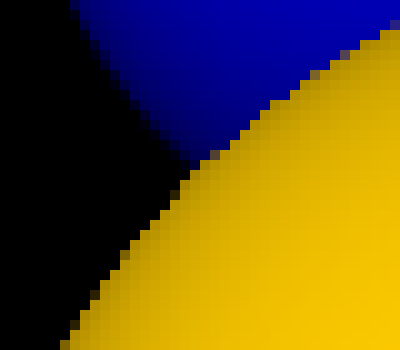
\includegraphics[width=\textwidth]{raytracer/zoomed-scene01-ss-ref.png}
			\end{figure}
		\end{column}
	\end{columns}
\end{frame}

\section{Solar system}
\begin{frame}
	\begin{figure}
		\includegraphics[width=\textwidth]{raytracer/solarsystem.png}
	\end{figure}
\end{frame}

\end{document}